\section{The Segment Routing (SR) architecture}
\label{sec:arch}

This section includes a short introduction to the main SR architectural aspects. Our goal is to provide a common ground and a reference conceptual framework for the survey, rather than to cover the details in a tutorial way.

The seminal paper on the Segment Routing Architecture is \cite{filsfils2015segment}. Published in 2014, it provides an overview of the motivations for SR, describes a set of important use cases and illustrates the architecture. The basic concepts proposed in \cite{filsfils2015segment} have been elaborated and refined in the RFC 8402 \cite{rfc8402} which has recently completed its standardization process in the IETF (July 2018). Obviously, RFC 8402 \cite{rfc8402} represents the most important source of information for the SR architecture. The work in \cite{sr-ietf-journal} (published in 2017) provides a short and effective introduction to the Segment Routing architecture, with focus on the MPLS dataplane. The survey paper \cite{abdullah2018segment} has a section about the SR architecture, which tries to give more details related to both the Data Plane and the Control Plane aspects.  

Following the RFC 8402, let us start by discussing the general concepts of SR, which are independent from the specific dataplane (MPLS or IPv6). An \textit{SR policy} is an ordered list of segments (segment list). As shown in Fig.~\ref{fig:sr_operations}, the segment list is added to the packet headers by a \textit{headend} node that \textit{steers} the packets of a flow onto the SR policy. A Segment Routing domain (\textit{SR domain}) is the set of nodes participating in the source-based routing model. The headend node can be the originator of the packet or (as Fig.~\ref{fig:sr_operations}) an intermediate node that performs a classification of the traffic and associates the SR policies to the packets. In other words, hosts \textit{can} be part of an SR domain, but this is not required and depends on the overall scenario in which SR is applied. It is expected that all nodes in an SR domain are managed by the same administrative entity. For example, a Service Provider backbone can constitute an SR domain and the headend node will be the ingress edge router of the backbone (in this case hosts are not part of the SR domain).

A segment is described by a Segment Identifier (\textit{Segment ID} or \textit{SID}). For the SR-MPLS dataplane, a SID is an MPLS label, while for the SR-IPv6 dataplane a SID is an IPv6 address. An SR policy P consisting in steering a packet along three segments with SIDs S1, S2 and S3 can be represented as P=<S1,S2,S3> (see Fig.~\ref{fig:sr_operations}). Three basic operations on SIDs and segment lists have been defined for a generic SR dataplane: PUSH, NEXT and CONTINUE. We assume for simplicity that S1, S2 and S3 represent topological instructions, so that the policy P instructs the packet to cross three nodes in sequence, identified by the SIDs S1, S2 and S3. 
%Note that these operations have been originally defined having the MPLS data plane in mind and then they can be remapped for the IPv6 dataplane.
The PUSH operation consists in the insertion of a segment on top of the segment list, i.e. as the new first segment of the SR policy. In order to build the SR policy P described above, the headend node executes the PUSH operations in this order: PUSH(S3), PUSH(S2), PUSH(S1). In an SR packet, the segment that specifies the instruction to be executed is called \textit{active} segment. In the considered example with the SR policy P, the headend node will send the packet with active segment S1. The NEXT operation is executed by a node that has processed the active segment and considers the next segment of the SR policy to be executed. In our example, the node identified with SID S1 receives the packet and perform the NEXT operation. The next segment is S2, which becomes the active segment and the packet is forwarded toward S2. The NEXT operation also covers the case of the last node of an SR policy, in which the NEXT operation usually results in processing the packet according to regular IP forwarding. The CONTINUE operation is performed by nodes that are in the path between two segments. For example, the intermediate nodes in the path between S1 and S2 perform the CONTINUE operation. The path between S1 and S2 is not prescribed by the SR policy and will be chosen considering the regular IP routing toward node S2 in the SR domain. If there are multiple equal cost paths between nodes S1 and S2 (as in Fig.~\ref{fig:sr_operations}) and the ECMP (Equal Cost MultiPath) mechanism is supported by the IP routing in the SR domain, it can be conveniently exploited by Segment Routing. 

\begin{figure}
    \centering
    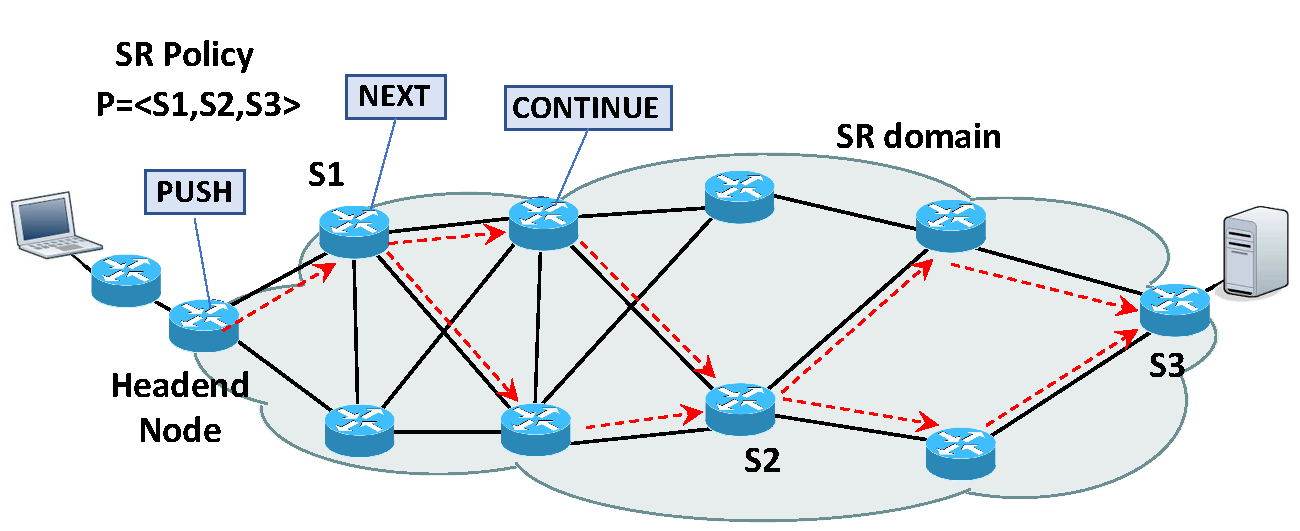
\includegraphics[width=0.45\textwidth]{fig/sr-domain.pdf}
    \caption{Example of an SR policy and of SR operations}
    \label{fig:sr_operations}
    \vspace{-3ex}
\end{figure}
%pdf generated by powerpoint, printing on PDF creator 
% settings, advanced settings, papersize postscript custom page setup
% width 95 mm height 240 mm % print quality 1200 dpi % true type download as softfonts
% in powerpoint settings "High quality" from the slides print setting


The segments can be classified into \textit{Global Segments} and \textit{Local Segments}. Global Segments correspond to instructions that are globally valid in an SR domain. Local segments correspond to instructions that are valid within a single node. The typical example of a global segment is an instruction to forward packets towards a given destination IP network or a destination IP node. Considering that an IGP (Interior Gateway Protocol) routing protocol (e.g. OSPF or ISIS) is used in the SR domain, these instructions are called \textit{IGP-prefix segment} and \textit{IGP-node segment} (or simply prefix segment and node segment). All nodes in the SR domain can execute the prefix segment or node segment instructions by considering the path towards the destination network or destination node in their own routing table. The most important example of local segment is the instruction to forward a packet to a node identified as adjacent by the IGP routing protocol. This corresponds to sending the packet on a specific outgoing interface and can be executed only on a specific node. This instruction is called \textit{IGP-Adjacency Segment}. Thanks to the use of IGP-Adjacency segments, it is possible to prove that any path across an SR domain can be expressed by an SR Policy (which can include a combination of global and local segments) \cite{pmsr}. Local segments can also be used to represent service instructions to be executed in a given node. The mapping of global and local segment into Segment Identifiers (SIDs) and the distribution of the SIDs in an SR domain are specific to the two different dataplanes (MPLS and IPv6) and will be discussed in the next subsections.

The \textit{IGP-Anycast Segment} is an IGP-Prefix segment that corresponds to an anycast prefix, i.e. a prefix advertised by a set of routers that can be used for High Availability or Load Balancing purposes. 

The \textit{Binding Segment} is used to associate an SR policy to a SID (called Binding SID or \textit{BSID}). A packet received with the BSID will be steered on the associated SR policy, this means that the packet will be forwarded using the corresponding Segment List. Using the Binding Segment it is possible to separate the processes of packet classification by the enforcing of a specific SR Policy. The SR policy can be changed over time (and can be executed in a different node) with no need to change the classification process. This improves the scalability, resilience and service independence of the solutions based on Segment Routing.

Segment Routing is supported by two different dataplanes: i) MPLS and ii) IPv6. Table~\ref{table-sr-mappings} summarizes the mapping of the SR concepts into the two dataplanes and will be discussed in the next two subsections. 

\begin{table}
\caption{\\Mapping SR concepts into SR-MPLS and SRv6}
\label{table-sr-mappings}
\begin{tabular}{|l|l|l|}
\hline
\textbf{Generic SR}                                          & \textbf{SR-MPLS} & \textbf{SRv6}                                                                                                                               \\ \hline
SR Policy                                                    & Label Stack      & \begin{tabular}[c]{@{}l@{}}Segment List (of IPv6\\ addresses) in the SR Header\end{tabular}                                                 \\ \hline
Active Segment                                               & Topmost Label    & \begin{tabular}[c]{@{}l@{}}IPv6 address indicated\\ by the Segment Left field\end{tabular}                                                  \\ \hline
\begin{tabular}[c]{@{}l@{}}PUSH\\ Operation\end{tabular}     & Label Push       & \begin{tabular}[c]{@{}l@{}}Adding an IPv6 in the Segment\\ List in the SR Header\end{tabular}                                               \\ \hline
\begin{tabular}[c]{@{}l@{}}NEXT\\ Operation\end{tabular}     & Label POP        & \begin{tabular}[c]{@{}l@{}}Decrementing the Segment Left\\ field, copying the active segment\\ in the IPv6 Destination Address\end{tabular} \\ \hline
\begin{tabular}[c]{@{}l@{}}CONTINUE\\ Operation\end{tabular} & Label Swap       & \begin{tabular}[c]{@{}l@{}}Forwarding according to IPv6\\ Destination Address\end{tabular}                                                  \\ \hline
\end{tabular}
\end{table}

\subsection{MPLS dataplane (SR-MPLS)}
\label{sec:mpls-dataplane}

The MPLS dataplane (SR-MPLS) is specified in \cite{id-segment-routing-mpls}. For SR-MPLS, Segment Routing does not require any change to the MPLS forwarding plane. An SR Policy is instantiated through the MPLS Label Stack: the Segment IDs (SIDs) of a Segment List are inserted as MPLS Labels. 
The classical forwarding functions available for MPLS networks allow implementing the SR operations. The PUSH operation corresponds to the Label Push function, i.e. pushing one or more labels on top of an incoming packet and then sending it out of a particular outgoing interface. The NEXT operation corresponds to the Label Pop function, i.e. removing the topmost label. The CONTINUE operation corresponds to Label Swap function, i.e. removing the incoming label and inserting an outgoing one. 
The encapsulation of an IP packet into a SR-MPLS packet is performed at the edge of an SR-MPLS domain if the destination address of the packet matches a pre-configured Forwarding Equivalent Class (FEC) associated with a specific SR Policy.

The mapping of Segments to MPLS Labels (SIDs) is a critical process in the SR-MPLS dataplane. In the general case, different routers in the SR domain could have different available ranges of labels to be used for Segment Routing. Therefore each router can advertise its own available label space to be used for Global Segments called \textit{SRGB - Segment Routing Global Block} (in general, this label space can even be composed of a set of non contiguous blocks). For this reason, in the SR domain the Global Segments are identified by an index, which has to be re-mapped into a label taking into account the node that will process the label. Assuming that the SRGB of a node is a label range starting from 10000, for a Global Segment with index X, the node needs to receive the label 10000+X. As an example, in Fig.~\ref{fig:mpls-dataplane}~A we consider how to implement the SR policy described in Fig.~\ref{fig:sr_operations} using the SR-MPLS dataplane in the general case in which different nodes are using different SRGBs. The SRGBs of the nodes and the segment index associated to the segments S1, S2 and S3 are shown in the gray rectangle. The headend node needs to consider in advance which is the SRGB of the nodes that will perform the NEXT operation the segments, because the label for the next segments needs to be crafted accordingly. In particular, the initial label for segment S2 set by the headend node will be 1002, i.e. the SRGB of node S1 (1000) plus the index for segment S2 (2). Node S1 will have to modify the label to 4002 if the packet is forwarded to node N4 (whose SRGB is 4000) or to label 6002 if the packet is forwarded to node N6 (whose SRGB is 6000). Both nodes N4 and N6 will remap (swap) the label to 2002 when forwarding the packets to S2. The initial label for node S3 set by the headend node is 2003, i.e. the SRGB of node S2 (2000) plus the index for segment S3 (3). This label will reach node S2 unmodified, then it will be properly processed by node S2 that will remap (swap) it considering the SRGB of the next hop in the path towards node S3. This remapping process complicates the operations and the troubleshooting. There are also services (e.g. involving anycast segments) that cannot be realized if different SRGBs are used by different nodes. For this reason, \cite{rfc8402} strongly recommends that an identical range of labels (SRGB) is used in all routers, so that a Global Segment will always be mapped to the same SID (MPLS label) in all nodes. In Fig~\ref{fig:mpls-dataplane}~B we present the mapping of the same SR policy described in Fig.~\ref{fig:sr_operations} under the suggested operating mode in which an identical SRGB is used in all nodes. We observe that the MPLS labels do not need to be remapped, so that the same label consistently identifies the same segment throughout the SR domain.

\begin{figure}
    \centering
    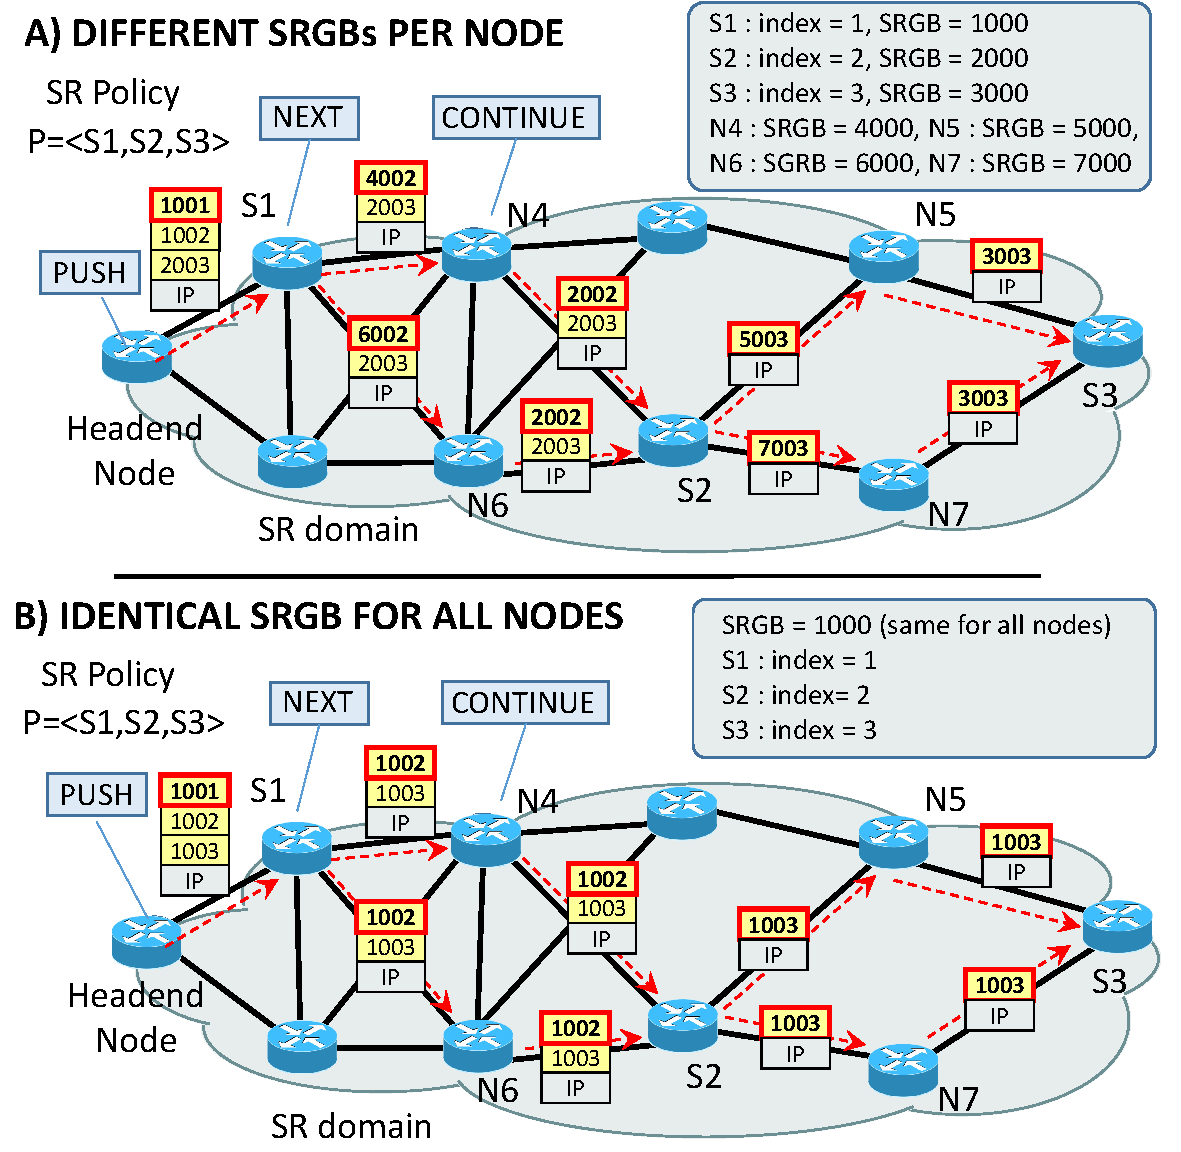
\includegraphics[width=0.48\textwidth]{fig/srgb-mpls-ok.pdf}
    \caption{SR-MPLS dataplane: mapping segments to labels using the SRGB}
    \label{fig:mpls-dataplane}
    \vspace{-3ex}
\end{figure}
%pdf generated by powerpoint, printing on PDF creator 
% settings, advanced settings, papersize postscript custom page setup
% width 195 mm height 200 mm % print quality 1200 dpi % true type download as softfonts
% in powerpoint settings "High quality" from the slides print setting


\subsection{IPv6 dataplane (SRv6)}
\label{sec:ipv6 dataplane}

For the IPv6 dataplane (SRv6), a new type of IPv6 Routing Extension Header, called Segment Routing Header (SRH) has been defined in \cite{ietf-6man-segment-routing-header}. The format of the SRH is shown in Fig.~\ref{fig:sr-header}. The SRH contains the Segment List (SR Policy) as an ordered list of IPv6 addresses: each address in the list is a SID. A dedicated field, referred to as \textit{Segments Left}, is used to maintain the pointer to the active SID of the Segment List. To explain the SRv6 dataplane, we consider three categories of nodes: Source SR nodes, Transit nodes and SR Segment Endpoint nodes. A Source SR node corresponds to the \textit{headend} node discussed above. It can be a host originating an IPv6 packet, or an SR domain ingress router encapsulating a received packet in an outer IPv6 header. In Fig.~\ref{fig:srv6-dataplane} we consider the latter case, the Source SR node is an edge router that encapsulates a packet (which can be IPv6, IPv4 or even a Layer 3 frame) into an outer IPv6 packet and inserts the SR Header (SRH) as a Routing Extension Header in the outer IPv6 header. The encapsulated packet is indicated as Payload in Fig.~\ref{fig:srv6-dataplane}. The Segment List in the SRH is composed of S1, S2 and S3 which are stored in reverse order (the fist SID is S3, the last segment in the SR policy). The Segment Left field is set to 2, so that the active segment is S1, represented in red in the figure. The Source SR node sets the first SID of the SR Policy (S1) as IPv6 destination address of the packet. These operations correspond to a sequence of the PUSH operations described above. The SR Segment Endpoint node receives packets whose IPv6 destination address is a local address of an interface or is locally configured as a segment. The SR Segment Endpoint node inspects the SR header: it detects the new active segment, i.e. the next segment in the Segment List, modifies the IPv6 destination address of the outer IPv6 header and forwards the packet on the basis of the IPv6 forwarding table. These operations correspond to the NEXT operation described above. In Fig.~\ref{fig:srv6-dataplane}, we can see that S1 is the first SR Endpoint node, it decrements the Segment Left fields to 1, making S2 the active segment, and sets S2 as IPv6 Destination Address. A Transit node forwards the packet containing the SR header as a normal IPv6 packet, i.e. on the basis of the (outer) IPv6 destination address, because the IPv6 destination address is not a local address, nor it has been configured as a segment. This behavior corresponds to the CONTINUE operation. In Fig.~\ref{fig:srv6-dataplane}, nodes N4, N5, N6 and N7 are Transit nodes, which perform a regular forwarding of the packet towards the IPv6 Destination Address. Note that in SRv6 the Transit nodes do not need to be SRv6 aware, as every IPv6 router can act as an SRv6 Transit node. 

\begin{figure}
    \centering
    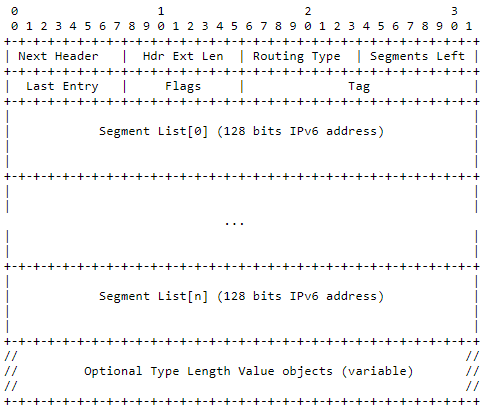
\includegraphics[width=0.8\columnwidth]{fig/sr-header.png}
    \caption{Segment Routing Header}
    \label{fig:sr-header}
%    \vspace{-3ex}
\end{figure}

\begin{figure}
    \centering
    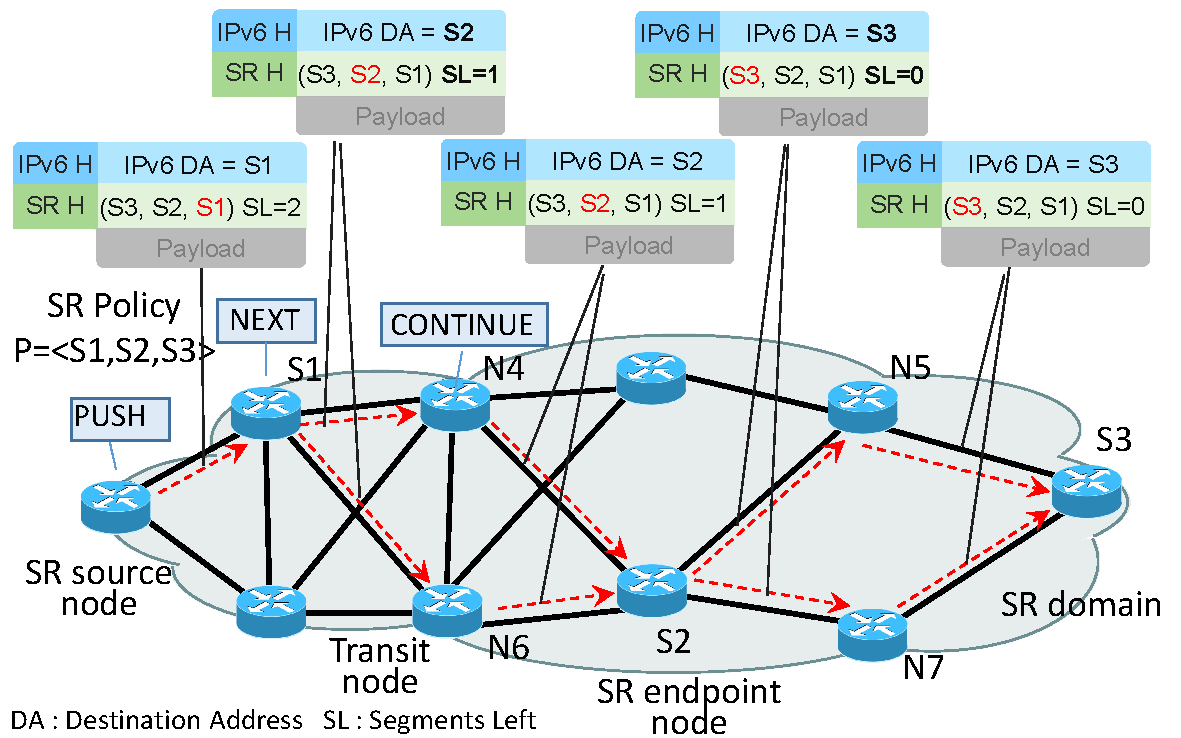
\includegraphics[width=0.48\textwidth]{fig/srv6-example.pdf}
    \caption{SRv6 dataplane operations}
    \label{fig:srv6-dataplane}
    \vspace{-3ex}
\end{figure}
%pdf generated by powerpoint, printing on PDF creator 
% settings, advanced settings, papersize postscript custom page setup
% width 118 mm height 230 mm % print quality 1200 dpi % true type download as softfonts
% in powerpoint settings "High quality" from the slides print setting

In the given example, the PUSH operation is performed by encapsulating a packet (IPv6, IPv4 or Layer 2 frame) into an outer IPv6 packet with a Segment Routing Header. Another possibility is to perform the \textit{insertion} of an SRH as a new header between the IPv6 header and the Next Header (e.g. the Trasport Layer Header, TCP or UDP), without encapsulating the packet in a new IPv6 packet. This option only applies to IPv6 packets and it is especially suited in case a host is acting as Source SR node (Headend node). 

In addition to the basic operations (PUSH/ NEXT/ CONTINUE), the \textit{SRv6 Network Programming} model \cite{id-srv6-network-prog} describes a set of functions that can be associated to segments and executed in a given SRv6 node. Examples of such functions are: different types of packet encapsulation (e.g. IPv6 in IPv6, IPv4 in IPv6, Ethernet in IPv6), corresponding decapsulation, lookup operation on a specific routing table (e.g. to support VPNs). A more complete list is provided in \cite{id-srv6-network-prog}, but the list is not meant to be exhaustive, as any function can be associated to a segment identifier in a node. Obviously, the definition of a standardized set of segment routing functions facilitates the deployment of SR domains with interoperable equipment from multiple vendors. 

According to \cite{id-srv6-network-prog}, we can revisit the notion of Segment IDentifier (SID) taking into account that IPv6 addresses are used as SIDs in SRv6. A 128 bit SID can be logically split in two fields and interpreted as LOCATOR:FUNCTION where LOCATOR includes the L most significant bits and FUNCTION the remaining 128-L least significant bits. The locator corresponds to an IPv6 prefix (e.g. with a length of 48 bits) that can be distributed by the routing protocols and provides the reachability of a node that hosts a number of functions. The length of the locator is not fixed and can be chosen by each operator for its own SR domain (also independently for different nodes). All the different functions residing in a node can share the same locator and have a different FUNCTION code, so that their SID will be different. From the routing point of view, the solution is very scalable as a single prefix is distributed, with limited impact on the routing tables of the nodes in the SR domain. The LOCATOR:FUNCTION representation of a SID can also be extended by splitting the FUNCTION field into FUNCTION:ARGUMENTS, so that the least significant bits can be used to provide information to a given function.

The concept of Network Programming consists in combining functions that can reside in different nodes to achieve \textit{a networking objective that goes beyond mere packet routing} \cite{id-srv6-network-prog}. The functions described in \cite{id-srv6-network-prog} can support valuable services and features like layer 3 and layer 2 VPNs, traffic engineering, fast rerouting. The Network Programming model offers the possibility to implement virtually any service by combining the basic functions in a \textit{network program} that can be embedded in the packet header. As shown in Fig.~\ref{fig:sr-header}, the SRH can include an optional section that carries Type Length Value (TLV) objects. These TLV objects can be defined to carry information that needs to be elaborated by one or more segments of an SR policy (Segment List). For example, the so-called HMAC TLV can be added and used to verify that an SRH header has been created by an authorized node and that the segment list is not modified in transit. Another potential use of TLV objects is for exchanging Operation and Maintenance (OAM) information among the nodes of the SR domain. 

% fast path vs slow path?

% My SID table ?

\subsection{Control plane for SR and relation with SDN}
\label{sec:sr_control_plane}

Control Plane operations are needed to complement the dataplane functionality and provide a complete solution for Segment Routing. The Control Plane can be based on a fully distributed approach, in which the routers are capable to take independent decisions to setup and enforce the SR Policies, it can rely on a centralized SR controller that takes decision and instructs the routers following the SDN principles, or on a combination of the two approaches (hybrid solution). 

For the SR-MPLS dataplane, the definition of a fully distributed approach has been worked out within the IETF, with the definition of extensions to the IGP routing protocols (OSPF, ISIS, see \cite{ietf-ospf-segment-routing-extensions} \cite{ietf-ospf-ospfv3-segment-routing-extensions} \cite{ietf-isis-segment-routing-extensions}). 
These extensions to the routing protocols are used by each routers to advertise the different types of IGP-segments (prefix, node, adjacency, anycast) and to distribute some SR configuration information. All other routers in the SR domain will receive this information by means of the IGP routing protocol. This information is needed to map the segments included in an SR policy into SIDs represented as MPLS labels in the SR-MPLS dataplane. As we have discussed in subsection \ref{sec:mpls-dataplane}, in the general case each router could allocate different ranges of labels to be used for Global Segments. The range of labels used for the global segments by a router, called \textit{SRGB - Segment Routing Global Block} is among the SR configuration information advertised using the routing protocol. We recall that it is strongly recommended to use an identical range of labels (SRGB) in all routers. 

For the IPv6 dataplane, the process of advertising the IGP-prefix, IGP-node and IGP-anycast segments is simplified thanks to the use of IPv6 addresses as SIDs. In particular, there is no need to extend the IGP routing protocols to distribute these segment types, represented as IPv6 prefixes that are natively distributed by the routing protocols. Also the definition of a Segment Routing Global Block as in the SR-MPLS is not needed and the operations related to Global Segments can rely on IPv6 addresses that are globally routable in the SR domain. This means that the Control Plane for SRv6 can use the regular IGP routing protocols (OSPF, ISIS) to support the basic operations, while extensions are still needed (\cite{id-isis-srv6-extensions} \cite{li-ospf-ospfv3-srv6-extensions}) to distribute IGP-Adjacency segments and other SR configuration information. 

The definition of the control plane for Segment Routing has started from the SR-MPLS dataplane and then the SRv6 dataplane has inherited most of the functionality, which has been adapted to the new dataplane. We observe that an original design goal of the control plane for Segment Routing has been to support the fully distributed approach, in which routers are capable to take autonomous decisions. This allows offering the the same functionality of a traditional MPLS network, which does not need a centralized SDN controller for its operations. On the other hand, we observe now a trend to focus on an hybrid approach, in which distributed routing protocols coexist with an SR controller. This hybrid approach is aligned with the vision of Software Defined Networking that aims at removing complexity from distributed nodes and to centralize control plane function in SDN controllers. In this light, the Segment Routing architecture can be deployed by seeking the right balance between distributed and centralized control. The distributed control is used by the routers to exchange reachability information and evaluate the shortest paths in a traditional way, with no need to interact with the centralized controller. We observe that this is the best approach to provide connectivity in Wide Area Networks in which the control connections between the nodes and the SDN controllers are affected by non-negligible latency and failure probability. Segment Routing can be used for Fast Reroute, by pre-configuring SR policies that provide alternate paths in case of link or node failures and are automatically activated by the node when the failure happens. The pre-calculation of such SR policies can be performed in a distributed mode or can be centralized in a controller. Basic topology information and additional information for Traffic Engineering need be conveyed to the controller, as well as service related information that is advertised by nodes using distributed routing protocols. The SDN controller can receive this information in different ways. For example, it can participate to the IGP routing protocol, it can interact with routers in a proprietary way to extract their IGP databases, it can receive information by routers using extensions to BGP-LS (BGP-Link State). Whatever mechanism has been used to retrieve the needed information from the nodes, the SDN controller is in charge to take decisions about the SR policies that implement advanced features or services like Traffic Engineering, VPNs or Service Function Chaining. This approach allows to clearly decouple the dataplane operations from the service logic operating in the control plane. The mechanisms and protocols for the SDN controller to enforce the SR policies by configuring the the nodes are left open in the SR architectural definition. As mentioned in \cite{rfc8402}, some options are Network Configuration Protocol (NETCONF), Path Computation Element Communication Protocol (PCEP) \cite{ietf-pce-segment-routing}, and BGP. The Openflow protocol can be used as a mechanism to configure the SR policies only for SR-MPLS, while SRv6 is not supported by the latest standard version of Openflow. An Open Source implementation of a SouthBound API for SRv6 based on gRPC is reported in \cite{ventre2018sdn}. The main characteristic of the Segment Routing solution compared to other SDN solutions is that only the edge nodes needs to be configured to enforce a given SR policy, while the internal nodes do not need to keep state per SR policy. This feature gives a substantial improvement in terms of scalability. 

\subsection{Segment Routing motivations and use cases}

As anticipated in the introduction section, the RFC 5439 \cite{rfc5439} has identified some scalability issues of traditional MPLS networks with Traffic Engineering support. These issues originated the interest in defining a more scalable solution like Segment Routing back in the late `00s. Several use cases and requirements for Segment Routing has been collected in a number of documents. In \cite{rfc7855}, the main use cases identified are: MPLS tunneling (i.e. to support VPN services), Fast ReRoute (FRR), Traffic Engineering (further classified in a number of more specific use cases). A set of Resiliency use cases is described in \cite{rfc8355}. In \cite{rfc8354}, the Segment Routing use cases for IPv6 networks are considered, with a set of exemplary deployment environments for SRv6: Small Office, Access Network, Data Center, Content Delivery Networks, Core Networks.

\begin{comment}
\begin{itemize}
      \item \cite{interconnecting} discusses the capability of SR-MPLS to interconnect a large number of end points with a limited SID space. 
\end{itemize}
\end{comment}



